\section{The Support Vector Machine}
The Support Vector Machine (SVM) is a supervised learning classifier originally designed for binary classifications. It was introduced by Vladimir N. Vapnik and Alexey Ya. Chervonenkis in 1963 \cite{Cortes1995}.

Let \( T := \{(\boldsymbol{x_1}, y_1),(\boldsymbol{x_2}, y_2),...,(\boldsymbol{x_n}, y_n)\} \),
be the training dataset, where $n$ is the number of the samples, \( \boldsymbol{x_i} \in \mathbb{R}^m \), \( i \in \{1,2,\dots,n\} \)
are samples, and \( y_i \in \{-1, 1\} \) are labels corresponding to samples \( \boldsymbol{x_i} \). The classification model is represented by the means of the hyperplane \( H \), defined such that:
\begin{equation}
    H: \boldsymbol{\omega}^T\boldsymbol{x}-\widetilde{b}=0,
    \label{eq:svm:hyperplane}
\end{equation}
where \( \omega \) is the normalized normal vector of the hyperplane \( H \), and
\begin{equation}
    \widetilde{b} = \frac{b}{\norm{\omega}}
    \label{eq:svm:offset}
\end{equation}
is the bias from the origin.

At first, we consider linearly separable training data. The two classes of data are distinguished by two hyperplanes such that the distance between them is maximized. The region bounded by these hyperplanes is called the margin. The hyperplane that lies halfway between them is called the maximum-margin hyperplane. These hyperplanes are described by the following equation:
\begin{equation}
    \boldsymbol{w}^T\boldsymbol{x}-\widetilde{b}=\pm1.
    \label{eq:svm_hyperplanes}
\end{equation}
Sample $x_i, i=1,\dots,n$ belongs to the positive class, i.e. $y_i = 1, i=1,\dots,n$, when
\begin{equation}
    \boldsymbol{w}^T\boldsymbol{x_i}-\widetilde{b}\geq1,
    \label{eq:svm_positive_data}
\end{equation}
and the negative class, i.e. $y_i = -1, i=1,\dots,n$, when
\begin{equation}
    \boldsymbol{w}^T\boldsymbol{x_i}-\widetilde{b}\leq-1.
    \label{eq:svm_negative_data}
\end{equation}
The properties \eqref{eq:svm_positive_data} and \eqref{eq:svm_negative_data} can be combined into a single equation
\begin{equation}
    y_i(\boldsymbol{w}^T\boldsymbol{x}-\widetilde{b})\geq1.
\end{equation}

\begin{figure}[ht!]
    \centering
    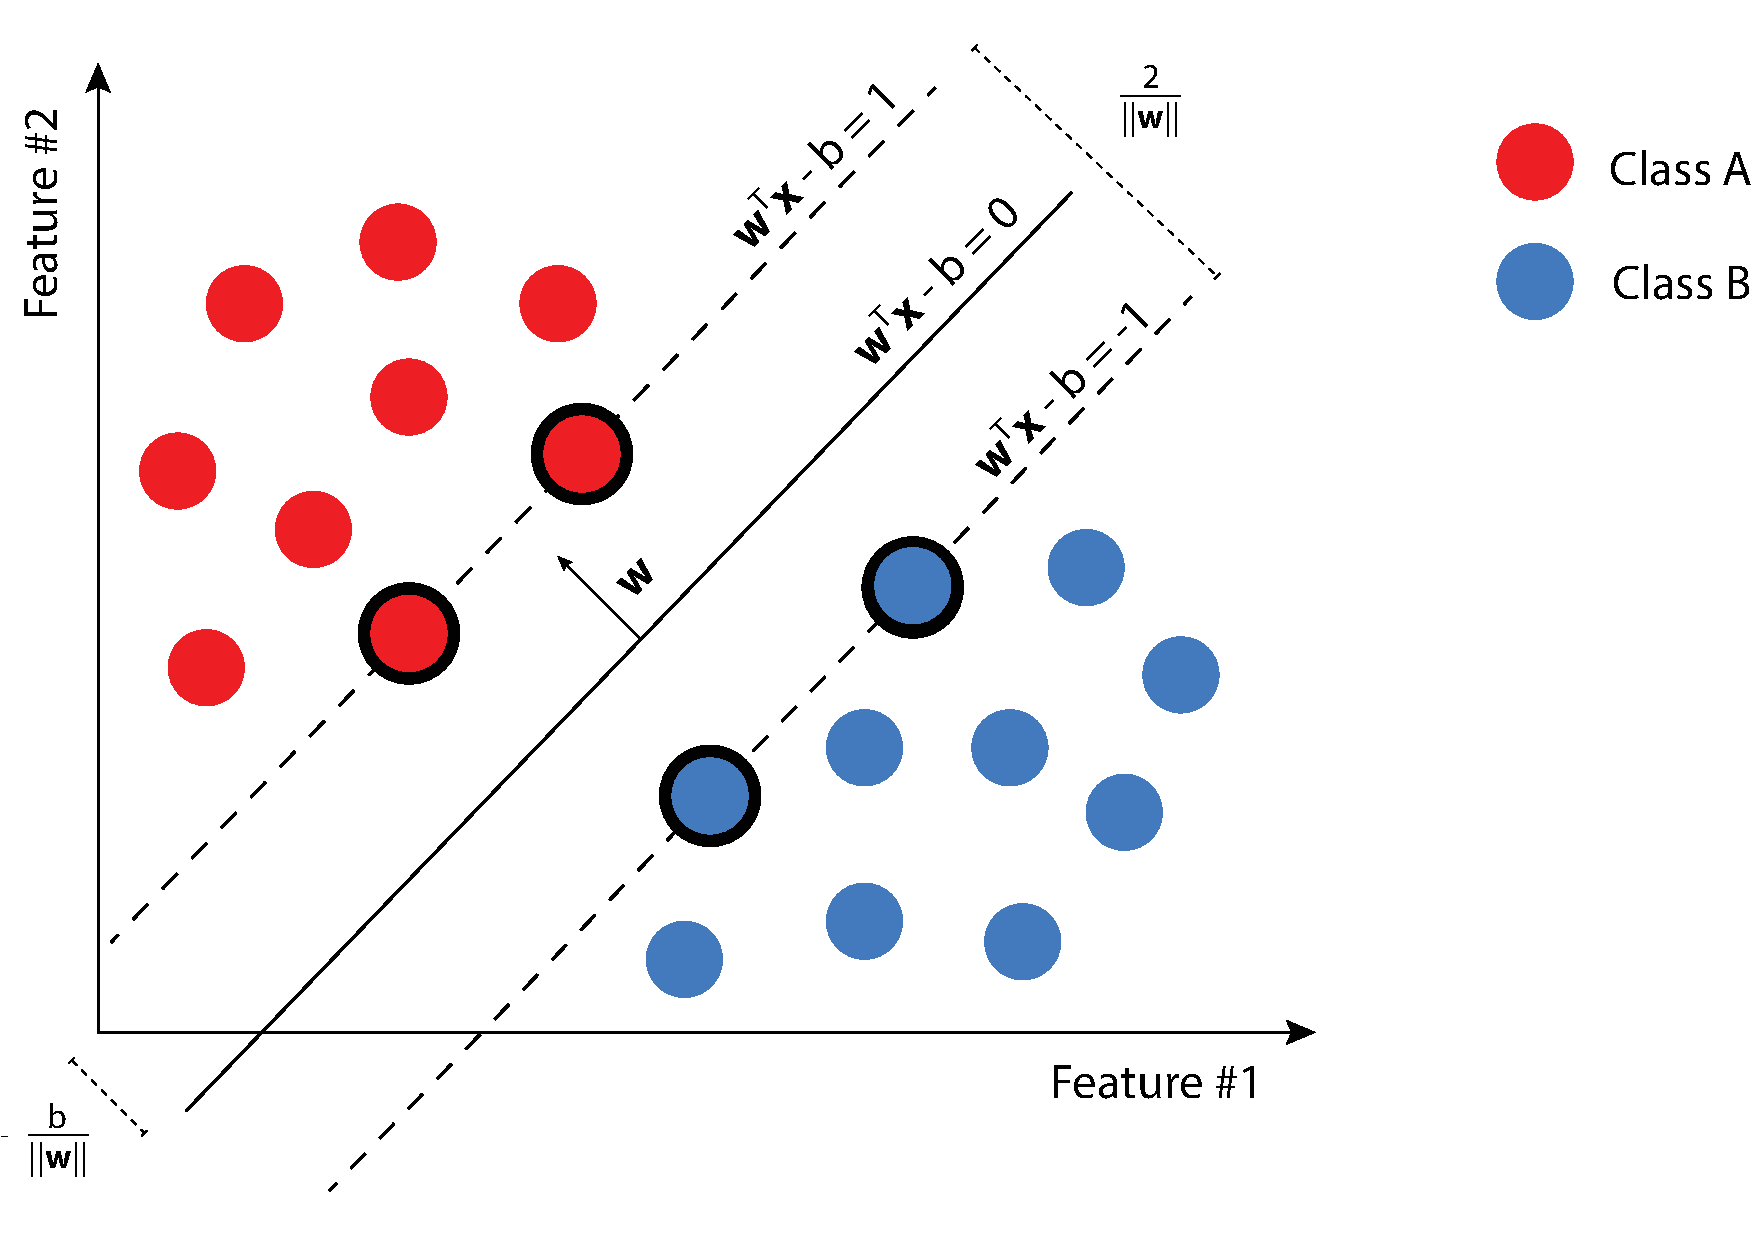
\includegraphics[width=0.65\textwidth]{Figures/svm/hyperplane_svm.pdf}
    \caption[Example of the SVM model]{Example of the SVM model \cite{Kruzik2018}.}
    \label{fig:svm-margin}
\end{figure}

From the \figref{fig:svm-margin}, we can see, the distance between hyperplanes \eqref{eq:svm_hyperplanes} is \( \frac{2}{\norm{\boldsymbol{w}}} \). Since we want to maximize this distance, we need to minimize $\norm{\boldsymbol{w}}$. This leads to an optimization problem
\begin{equation}
    \argmin_{\boldsymbol{w},b} \|\boldsymbol{w}\|\quad \text{ s.t. }
    \begin{cases}
        y_i(\boldsymbol{w}^T\boldsymbol{x}_i-b)\geq1,\\
        i=1, ...,n,
    \end{cases}
\end{equation}
which can be reformulated as the Quadratic Programming problem
\begin{equation}
    \argmin_{\boldsymbol{w},b} \frac{1}{2}\|\boldsymbol{w}\|^2\quad \text{ s.t. }
    \begin{cases}
        y_i(\boldsymbol{w}^T\boldsymbol{x}_i-b)\geq1,\\
        i=1, ...,n.
    \end{cases}
    \label{eq:svm_hard_margin_minimization}
\end{equation}

Because the training data is not commonly separable, the soft margin version of the SVM was proposed by Vladimir N. Vapnik and Corinna Cortes \cite{Cortes1995} in 1995. It exploits an additional function called the hinge loss function:
\begin{equation}
    \xi_i = \max(0, 1-y_i(\boldsymbol{w}^T\boldsymbol{x}_i-b)).
    \label{eq:svm_hinge_loss}
\end{equation}

The hinge loss function \eqref{eq:svm_hinge_loss} equals $0$ for a sample on the correct side of the corresponding hyperplane \eqref{eq:svm_hyperplanes}. However, for a sample on the wrong side of the corresponding hyperplane \eqref{eq:svm_hyperplanes}, the value of the function is proportional to the distance from the hyperplane.

If we add the hinge loss function \eqref{eq:svm_hinge_loss} to optimization problem \eqref{eq:svm_hard_margin_minimization}, we get a soft margin SVM optimization problem
\begin{equation}
    \argmin_{\boldsymbol{w},b,\xi_i} \frac{1}{2}\|\boldsymbol{w}\|^2 + C\sum_{i = 1}^n\xi_i\quad \text{ s.t. }
    \begin{cases}
        y_i(\boldsymbol{w}^T\boldsymbol{x}_i-b)\geq1 - \xi_i,\\
        \xi_i \geq 0 , i=1, ...,n,
    \end{cases}
    \label{eq:svm:soft_margin_minimization}
\end{equation}
where \( C \geq 0 \) is a penalty for the misclassification error. The formulation \eqref{eq:svm:soft_margin_minimization} is called the $l1$-loss $l2$-regularized SVM. The primal formulation \eqref{eq:svm:soft_margin_minimization} can be modified using the Lagrange duality with Lagrange multipliers $\boldsymbol{\alpha} = [\alpha_1, \alpha_2, ..., \alpha_n]^{\top}$, and $\boldsymbol{\beta} = [\beta_1, \beta_2, ..., \beta_n]^{\top}$ corresponding to inequality constraints. Exploiting Karush-Kuhn-Tucker conditions, we obtain the dual formulation
\begin{equation}
    \argmin_{\boldsymbol{\alpha}} \frac{1}{2} \boldsymbol{\alpha}^T\boldsymbol{Y}^T\boldsymbol{K}\boldsymbol{Y}\boldsymbol{\alpha} - \boldsymbol{\alpha}^T\boldsymbol{e}\quad \text{ s.t. } 
    \begin{cases}
        \boldsymbol{o} \leq \boldsymbol{\alpha} \leq C\boldsymbol{e},\\
        \boldsymbol{B_e}\boldsymbol{\alpha}=0,
    \end{cases}
    \label{eq:svm:soft_margin_dual}
\end{equation}
where \( \boldsymbol{e} = [1,1, \dots,1]^{\top} \), \( \boldsymbol{o} = [0,0, \dots,0]^{\top} \), \( \boldsymbol{X} = [\boldsymbol{x_1},\boldsymbol{x_2}, \dots,\boldsymbol{x_n}] \), \( \boldsymbol{y} = [y_1,y_2, \dots,y_n]^{\top} \), \( Y = \text{diag}(\boldsymbol{y}) \), \( \boldsymbol{B_e} = [\boldsymbol{y}^T] \), and \( \boldsymbol{K}\coloneqq\boldsymbol{X}^T\boldsymbol{X} \) is the Gram matrix which is symmetric positive semi-definite (SPSD) \cite{Aeta2018}. The Hessian matrix in \eqref{eq:svm:soft_margin_dual}
\begin{equation}
    \boldsymbol{H} \coloneqq \boldsymbol{Y}^T\boldsymbol{X}^T\boldsymbol{X}\boldsymbol{Y}
    \label{eq:svm:hessian}
\end{equation}
is also an SPSD matrix.

To recover the normal vector, the formula
\begin{equation}
    \boldsymbol{w}=\boldsymbol{X}\boldsymbol{Y}\boldsymbol{\alpha}.
    \label{eq:svm:dual_to_primal_w}
\end{equation}
is used. The bias $b$ can be recovered as
\begin{equation}
    b=\boldsymbol{w}\cdot \boldsymbol{\Bar{x}} - y_i,
    \label{eq:svm:dual_to_primal_b}
\end{equation}
where $\boldsymbol{\Bar{x}}$ is the mean of all support vectors.

Instead of the linear sum of the loss functions $\xi_i$ in \eqref{eq:svm:soft_margin_minimization}, we can use the square sum of the loss functions in the objective function
\begin{equation}
    \argmin_{\boldsymbol{w},b,\xi_i} \frac{1}{2}\|\boldsymbol{w}\|^2 + \frac{C}{2}\sum_{i = 1}^n\xi_i^2 \text{ s.t. } 
    \begin{cases}
        y_i(\boldsymbol{w}^T\boldsymbol{x}_i-b)\geq1 - \xi_i,\\
        i=1, ...,n.
    \end{cases}
    \label{eq:svm:soft_margin_minimization_l2}
\end{equation}
The problem \eqref{eq:svm:soft_margin_minimization_l2} is called $l2$-loss $l2$-regularized SVM. The dual formulation can again be obtained by using the Lagrange duality:
\begin{equation}
    \argmin_{\boldsymbol{\alpha}} \frac{1}{2} \boldsymbol{\alpha}^T(\boldsymbol{H}+C^{-1}\boldsymbol{I})\boldsymbol{\alpha} - \boldsymbol{\alpha}^Te \text{ s.t. } 
    \begin{cases}
        \boldsymbol{o} \leq \boldsymbol{\alpha},\\
        \boldsymbol{B_e}\boldsymbol{\alpha}=0.
    \end{cases}
    \label{eq:svm:soft_margin_dual-l2}
\end{equation}

In this case, the Hessian matrix $\boldsymbol{H}$, regularized by the matrix $C^{-1}\boldsymbol{I}$ is symmetric positive definite, therefore, this optimization problem should be more stable than the $l1$-loss $l2$-regularized SVM problem.

\subsection{Hyperparameter optimization}
Hyperparameter optimization is the process of selecting suitable parameters for a classifier. In SVM, we need to find an optimal penalty $C$. One approach of hyperparameter optimization is a Grid search.

Grid search is an exhaustive searching through a user-specified subset of parameters. The classifier is trained with each combination of the subset. The combination, which yields the best result is then selected. By the best result, we mean the highest score of a user-specified metric.

To test the hyperparameter selection, we need new, independent data from the data used in a training step. This is accomplished by splitting the data into subsets. The subsets are selected using a stratified cross-validation technique.

\subsection{Cross-validation}
Cross-validation is an approach to split a dataset into a training and validation subset \cite{RodPerLoz10}. For each set of hyperparameters, a dataset is split into $k$ subsets (folds) of an equal size. One of the subsets is kept as a validation set, while the model is trained on the other $k-1$ folds. The process is repeated $k$ times, selecting each fold as a validation subset. The results of all $k$ runs are averaged for a final score. This process is demonstrated in \figref{fig:k-fold}.
\begin{figure}
    \centering
    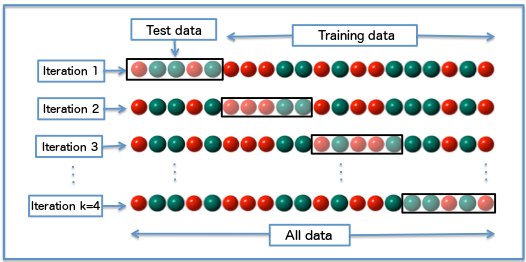
\includegraphics[width=0.7\textwidth]{Figures/svm/k-fold.jpg}
    \caption[$k$-fold cross-validation splits data into $k$ folds and trains the model $k$ times always leaving out a different fold as a validation set]{$k$-fold cross-validation splits data into $k$ folds and trains the model $k$ times always leaving out a different fold as a validation set \cite{crossval}.}
    \label{fig:k-fold}
\end{figure}

Since a randomly selected fold might not represent the classes in the same ratio as the whole set, stratified cross-validation is used. The random folds are selected in a way, where the ratio of the classes is roughly equal to the ratio of classes in the whole dataset.
